\documentclass[11pt]{article}
\usepackage[top=0.75in, bottom=0.5in, left=0.75in, right=0.75in]{geometry}
\usepackage{amsmath,amsfonts, color, booktabs, centernot, textcomp,amssymb,graphicx,verbatim,enumerate, bbm}
\usepackage{tabulary}
%\usepackage [autostyle, english = american]{csquotes}
%\usepackage [style = american]{csquotes}
%\MakeOuterQuote{"}
\usepackage{algorithm} % Boxes/formatting around algorithms
\usepackage[noend]{algpseudocode} % Algorithms
\usepackage{wrapfig}
\usepackage{fancyhdr}
\pagestyle{fancy}
\setlength\parindent{0pt}
%\newcounter{problemnumber}
\def\Name{Leah Dickstein}  % Your name

\title{\vspace{-5ex} CSoI Mid-Year Report}
\author{\Name \\
Mentored by: Gireeja Ranade, Anant Sahai \vspace{-2ex}}
\date{}
\lhead{CSoI Mid-Year Report: \Name}


\begin{document}
\maketitle

What I've been exploring is how time, delay and quantization affects information flows in a control system.

\subsection*{Problem Setup}
%At the end of Spring 2015, the problem setup was as follows:\\
\begin{minipage}{0.4\textwidth}
\begin{center}
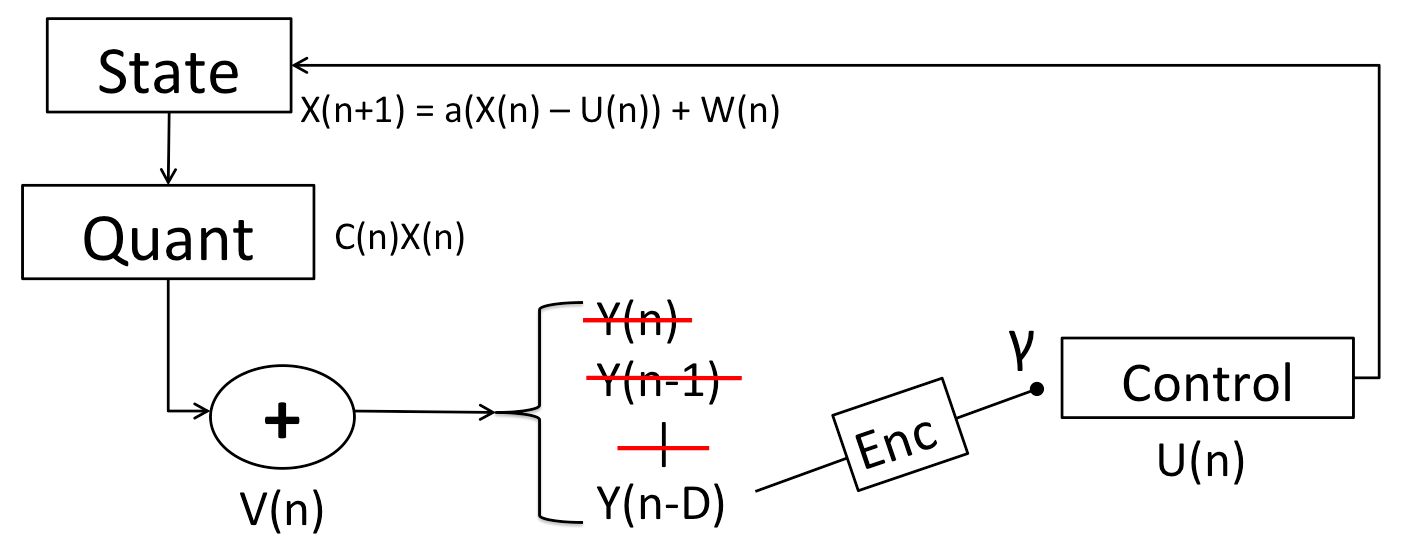
\includegraphics[width=0.7\textwidth]{sys_dynamics} 
\end{center}
\end{minipage}
\begin{minipage}{0.5\textwidth}
\[ X(n+1) = a(X(n) - U(n)) + W(n) \]
\[ Y(n) = \left\{
     \begin{array}{ll}
       Q(X(n)) + V(n) & : n \equiv 0 \text{ (mod D + 1)}\\
       0 & : \text{else}
     \end{array}
   \right. \]
\[ Q(X(n)) = C(n)X(n) \]
\[ U(n) = \left\{
     \begin{array}{ll}
       L[X(n) \; | \; Y(n-D)] & : n \equiv 0 \text{ (mod  D + 1)}\\
       0 & : \text{else}
     \end{array}
   \right. \]
\end{minipage}\\

%An optimal controller is defined to be one that minimizes the cost function, which was the second moment of the state.\\
% Why?
The state is a random variable with some unstable system gain, which is observed with some AWGN and encoded and sent across a BEC to the controller. We choose to model the number of bits in the observation encoding as a linear function of delay, which is then represented as quantization noise in the observation. We use an adaptive quantizer, thus quantization noise is modeled as multiplicative noise. Encoding is done via a Reed Solomon scheme.

%\subsection*{Observation Decoding Probability Correction}
%
%The probability was originally calculated as if each bit in the message (state) was dropped independently with probability $\frac{1}{2}$, and dropping too many bits would lead to packet corruption. This was an incorrect model, as Reed Solomon encoding actually works like a balls and bins setup with a binomial distribution. The packet decoding probability at the controller was corrected: $\gamma = 1-2^{-((1-R) \, m+1)} \rightarrow$ 1 $-$ ccdf(number of bits, 0.5). This resulted in the following plot correction:\\
%
%\begin{minipage}{0.5\textwidth}
%\begin{center}
%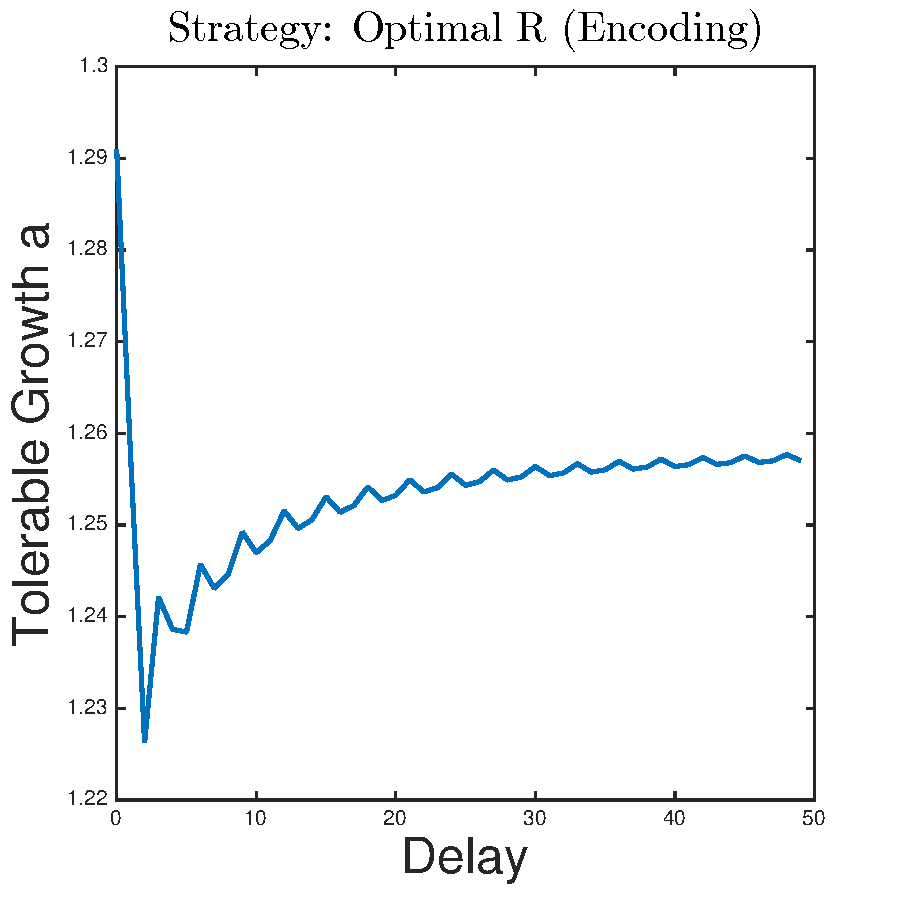
\includegraphics[width=0.8\textwidth]{150430_Dvsa}\\
%Spring 2015: $\gamma = 1-2^{-((1-R) \, m+1)} $
%\end{center}
%\end{minipage}
%\begin{minipage}{0.5\textwidth}
%\begin{center}
%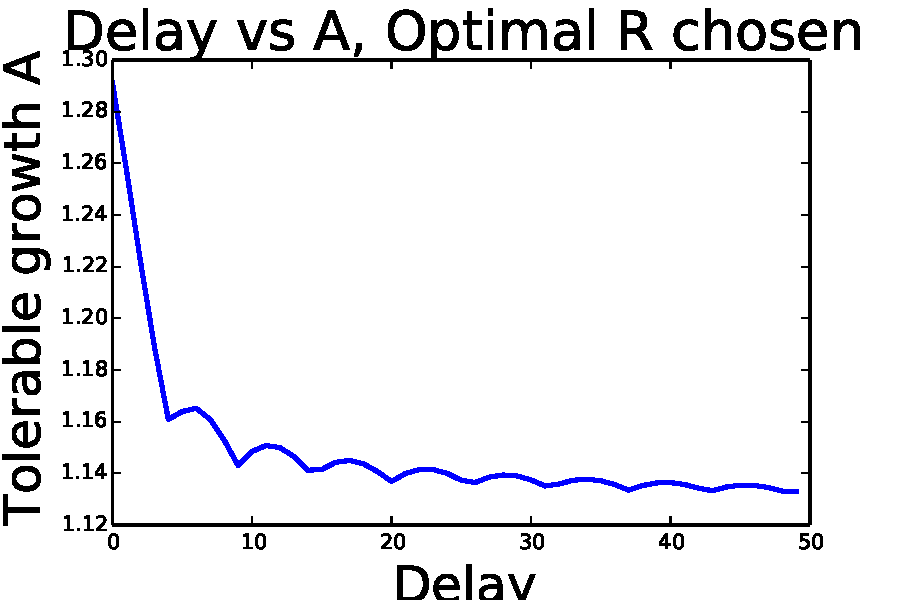
\includegraphics[width=0.8\textwidth]{binomial_delayvsa}\\
%Fall 2015: $\gamma =$ 1 $-$ ccdf(number of bits, 0.5)
%\end{center}
%\end{minipage}

\subsection*{Exploring Bounded Control Capacity}
I explored this problem framework under various cost functions. The question of interest was: is delay always bad? The first cost function minimizes the second moment of the state, while the second cost function also bounds the control capacity by penalizing control power. For simplicity, we chose an observation that had quantization noise but no AWGN. I obtained the following result:\\
\begin{minipage}{0.5\textwidth}
\[  \text{min } \mathbb{E}[x^2(n+1)] + \sum_{k=1}^n \, a^2 u^2(k) \]
\[ \alpha(n) = \frac{a^D \mu_c}{2(\mu_c^2 + \sigma_c^2)} \]
\[ a^{2(D+1)} \left( \frac{\mu_c^2 + 4\sigma_c^2}{4(\mu_c^2 + \sigma_c^2)} \right) < 1 \]
\end{minipage} \begin{minipage}{0.5\textwidth}
\begin{center}
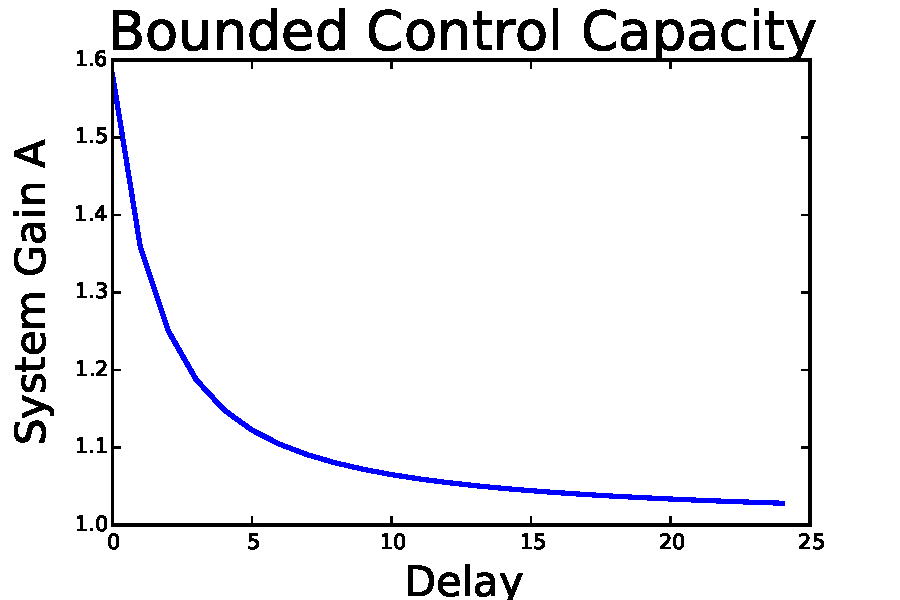
\includegraphics[width=0.8\textwidth]{160131_newcost}
\end{center}
\end{minipage}

%{\renewcommand{\arraystretch}{1.75}%
%\begin{tabulary}{\textwidth}{CC}
%min $\mathbb{E}[x^2(n+1)]$ & min $\mathbb{E}[x^2(n+1)] + \sum_{k=1}^n \, a^2 u^2(k)$ \\
%$\alpha(n) = \frac{a^D \mu_c}{\mu_c^2 + \sigma_c^2}$ & $\alpha(n) = \frac{a^D \mu_c}{2(\mu_c^2 + \sigma_c^2)}$ \\
%$a^{2(D+1)} \left( \frac{\sigma_c^2}{\mu_c^2 + \sigma_c^2} \right) < 1$ & $a^{2(D+1)} \left( \frac{\mu_c^2 + 4\sigma_c^2}{4(\mu_c^2 + \sigma_c^2)} \right) < 1$ \\
%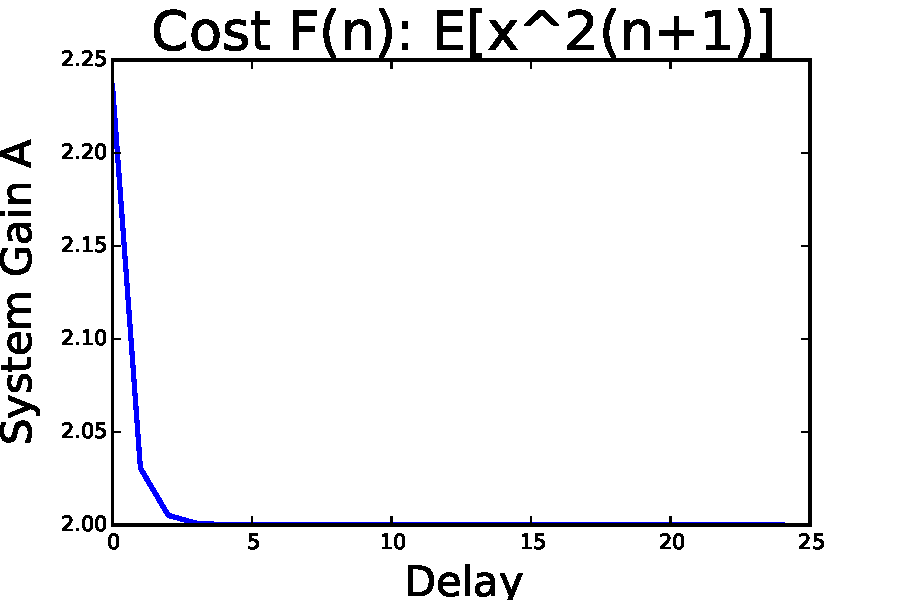
\includegraphics[width=0.4\textwidth]{160131_oldcost} & 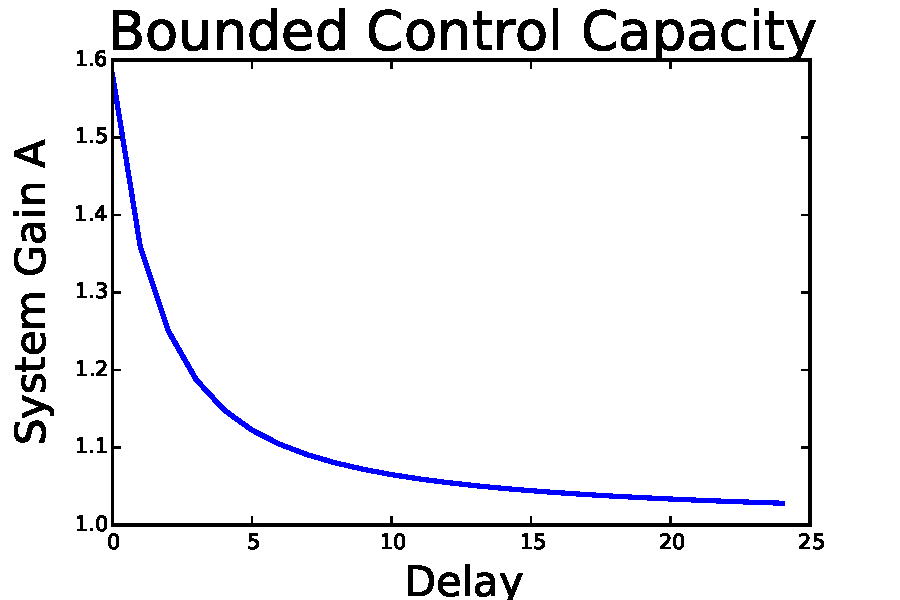
\includegraphics[width=0.4\textwidth]{160131_newcost}
%\end{tabulary}
%{\renewcommand{\arraystretch}{1}%

The control is the optimal linear memoryless controller $u(n) = \alpha(n) \, y(n-D)$. A is the maximum system gain where the state remains mean square stabilizable. The result makes sense, as the control ``sacrifices'' resolution of the state in exchange for reducing the power of the control. The result confirms that increasing delay is monotonically bad, even with different cost functions.

%Although this could be explored further, initial results appear negative.
%Something to be explored is whether our current bound is too loose (as is reflected in the left plot.)

% $\mathbb{E}[x^2(n+1)] \rightarrow \mathbb{E}[x^2(n+1)] + \sum_{k=1}^n \, u^2(k)$.

%\subsection*{Exploring Memory-Based Controller}
%
%From Gireeja Ranade's work\footnote{Gireeja Ranade and Anant Sahai. Non-Coherence in Estimation and Control. Allerton 2013.}, it can be shown that the optimal controller for a delay = 0 case is memoryless. This arises naturally from the control theoretic aspects of the problem; in this setup, the state is the error and thus the state is orthogonal to previous observations at every timestep. (I have a proof that the state is orthogonal to previous observations for both the optimal linear and optimal nonlinear controllers.) In addition, the problem can be modeled as a Hidden Markov Model which has the memoryless property. This memorylessness is not necessarily true for a setup with delay, where observations accumulate before a control is applied. \\
%
%If the cost function is $\mathbb{E}[x^2(n+1)]$, the optimal linear controller with the $D+1$ last observations is the LLSE:
%\[ U(n) = \left\{
%     \begin{array}{ll}
%       L[X(n) \; | \; \vec{Y}] & : n \equiv 0 \text{ (mod  D + 1)}\\
%       0 & : \text{else}
%     \end{array}
%   \right. \quad \quad L[X(n) \; | \; \vec{Y}] = \Sigma_{YY}^{-1} \, cov(x(n), \vec{Y}) \, \vec{Y} \]
%%\[ L[X(n) \; | \; \vec{Y}] = \frac{cov(x(n), \vec{Y})}{\Sigma_{YY}} \, \vec{Y} \]
%\[ \vec{Y} \doteq \begin{bmatrix}
%y(n) & y(n-1) & \cdots & y(n-D)
%\end{bmatrix}^T \]
%\[ cov(x(n), \vec{Y}) \doteq \begin{bmatrix}
%\mathbb{E}[x(n)y(n)] & \mathbb{E}[x(n)y(n-1)] & \cdots & \mathbb{E}[x(n)y(n-D)]
%\end{bmatrix} \]

\subsection*{Future Work: Spring 2016}
\begin{itemize}
\item I am currently working on a memory-based controller, and may pursue nonlinear controllers. %I have the control vector $\vec{\alpha}(n)$ calculated, but still need to upper bound system gain (where the state is mean square stabilizable.) Where I proceed is dependent on this result.

\item I am also looking at how wireless protocols interact with control.

% \item I  want to explore how a one timestep increase in delay affects one timestep of system growth. This will help me explore how observation message length connects to the number of bits in the state that I can control.

% With the observation decoding probability correction, I want to explore how the encoding rate has changed with the new probability distribution.
% 

%\item If memory-based controller fails, I \textit{may} consider exploring nonlinear controllers. Quantization noise is multiplicative, so the observation is no longer Gaussian. The MMSE is not necessarily linear.
%\item I probably won't explore different encoding schemes, but I \textit{do} need to better understand the finite blocklength aspects of this problem.
%\item If memory-based and select nonlinear controllers result in delay vs system gain as a monotonically decaying curve, I may pursue proving that delay will always be negatively correlated with system gain. This needs to be discussed with my mentors.
\end{itemize}

\end{document}